\begin{figure}[htb]
\centering
\includegraphics[page=6,width=0.45\textwidth]{\FCNCFigures/tthML/raw/faketau/prefit/NOMINAL/reg1l1tau1b1j_ss_vetobtagwp70_highmet/tau_pt_0.pdf}
\put(-100, 140){\textbf{(a)}}
\put(-120, 130){\footnotesize{$l\thad 1j$}}
\includegraphics[page=6,width=0.45\textwidth]{\FCNCFigures/tthML/raw/faketau/prefit/NOMINAL/reg1l1tau1b2j_ss_vetobtagwp70_highmet/tau_pt_0.pdf}
\put(-100, 140){\textbf{(b)}}
\put(-120, 130){\footnotesize{$l\thad 2j$}}

\includegraphics[page=6,width=0.45\textwidth]{\FCNCFigures/tthML/raw/faketau/prefit/NOMINAL/reg1l1tau1b2j_os_vetobtagwp70_highmet/tau_pt_0.pdf}
\put(-100, 140){\textbf{(c)}}
\put(-120, 130){\footnotesize{$STH \tlhad OS$}}
\includegraphics[page=6,width=0.45\textwidth]{\FCNCFigures/tthML/raw/faketau/prefit/NOMINAL/reg1l1tau1b3j_os_vetobtagwp70_highmet/tau_pt_0.pdf}
\put(-100, 140){\textbf{(d)}}
\put(-120, 130){\footnotesize{$TTH \tlhad OS$}}

\includegraphics[page=6,width=0.45\textwidth]{\FCNCFigures/tthML/raw/faketau/prefit/NOMINAL/reg1l2tau1bnj_os/tau_pt_0.pdf}
\put(-100, 140){\textbf{(e)}}
\put(-120, 130){\footnotesize{$l\thadhad OS$}}

\caption{ The distributions of $\tau$ $\pt$ in the signal regions. }
\label{fig:pt_raw}
\end{figure}
